\documentclass[tikz, border=1mm]{standalone}
\usetikzlibrary{positioning}

% Source: https://tex.stackexchange.com/a/24133/45450
\makeatletter
\newcommand*{\textoverline}[1]{$\overline{\hbox{#1}}\m@th$}
\makeatother

\begin{document}
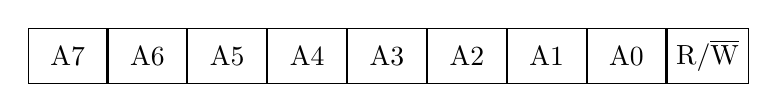
\begin{tikzpicture}
\node (A7) [draw, minimum height=7mm, minimum width=10mm] {A7};
\node (A6) [draw, minimum height=7mm, minimum width=10mm, right=0cm of A7] {A6};
\node (A5) [draw, minimum height=7mm, minimum width=10mm, right=0cm of A6] {A5};
\node (A4) [draw, minimum height=7mm, minimum width=10mm, right=0cm of A5] {A4};
\node (A3) [draw, minimum height=7mm, minimum width=10mm, right=0cm of A4] {A3};
\node (A2) [draw, minimum height=7mm, minimum width=10mm, right=0cm of A3] {A2};
\node (A1) [draw, minimum height=7mm, minimum width=10mm, right=0cm of A2] {A1};
\node (A0) [draw, minimum height=7mm, minimum width=10mm, right=0cm of A1] {A0};
\node (RW) [draw, minimum height=7mm, minimum width=10mm, right=0cm of A0] {R/\textoverline{W}};
\end{tikzpicture}
\end{document}